\documentclass[final,5p,times,twocolumn,authoryear]{report}
\usepackage[a4paper,left=2cm,right=2cm,includehead,nomarginpar,textwidth=10cm,headheight=14pt]{geometry}

\usepackage{amssymb}
\usepackage{amsthm}
\usepackage{amsmath}
\usepackage[utf8]{inputenc}
\usepackage{lineno}
\usepackage{tabularx}
\usepackage{graphicx}

\newcommand{\pd}[2]{\frac{\partial #1}{\partial #2}}
\newcommand{\pdd}[2]{\frac{\partial^2 #1}{\partial #2^2}}


\begin{document}

\begin{titlepage}
   \begin{center}
   		
\includegraphics[width=0.2\textwidth]{UGA-logo}
   		
       \vspace*{1cm}

       \textbf{Caractérisation des sources d'incertitudes associées à un ensemble de simulations stochastiques de la circulation océanique
tourbillonnaire dans l'Océan Indien Sud-Ouest}
                    
       \vfill
       
       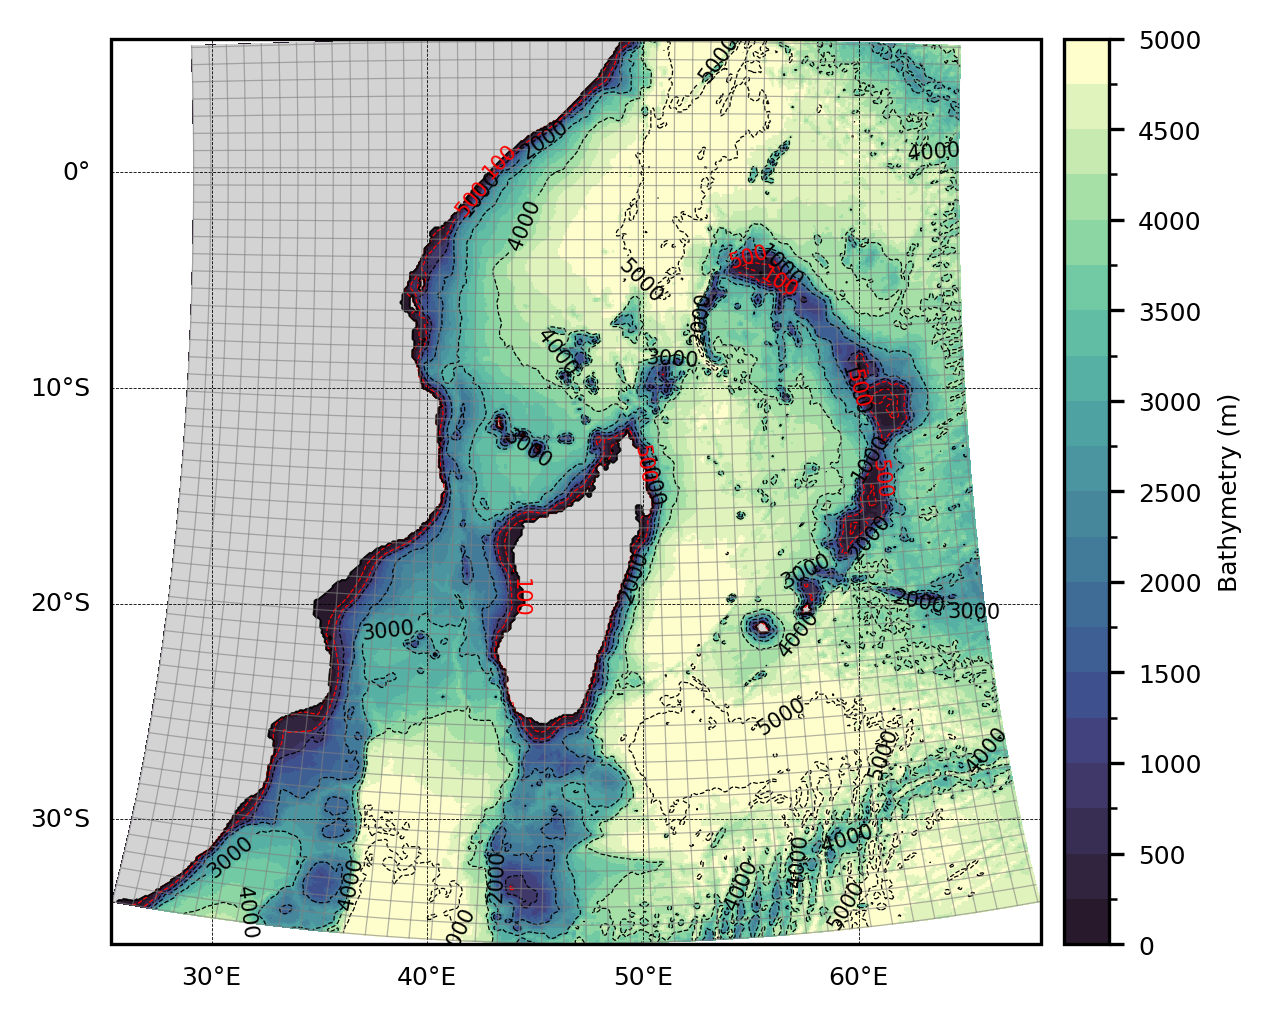
\includegraphics[width=0.9\textwidth]{figures/bathy_iso_swio2_grid.png} 
       %\captionof{}{}
       
       \vfill
       
       \textbf{Rémy Guillermin}
       
       \vspace{0.5cm}
        Supervisé par Pierre Brasseur, Jean-Michel Brankart et Lisa Weiss
            
       \vspace{0.8cm}

       2024-2025
            
   \end{center}
\end{titlepage}




\end{document}